\documentclass[12pt]{article}
\usepackage[margin=1in]{geometry}% Change the margins here if you wish.
\usepackage{amsmath,amsthm,amssymb,stmaryrd}
\usepackage[english]{babel}
\setlength{\parindent}{0pt} % This is the set the indent length for new paragraphs, change if you want.
\setlength{\parskip}{5pt} % This sets the distance between paragraphs, which will be used anytime you have a blank line in your LaTeX code.
\usepackage[textwidth=1.9cm,textsize=small]{todonotes}
\usepackage{hyperref}
\usepackage{tikz}
\usetikzlibrary{automata, positioning, arrows}
\tikzset{
    ->, % makes the edges directed
    >=stealth, % makes the arrow heads bold
    node distance=3cm, % specifies the minimum distance between two nodes. Change if necessary.
    every state/.style={thick, fill=gray!10}, % sets the properties for each ’state’ node
    initial text=$ $, % sets the text that appears on the start arrow
    }

\newcommand{\ifilip}[1]{\todo[inline,color=green!10]{{\bf Filip:} #1}}
\newcommand{\filip}[1]{\todo[color=green!10]{{\bf Filip:} #1}}

\newcommand{\iolek}[1]{\todo[inline,color=red!10]{{\bf Olek:} #1}}
\newcommand{\olek}[1]{\todo[color=red!10]{{\bf Olek:} #1}}


\newcommand{\icol}[1]{% inline column vector
  \left(\begin{smallmatrix}#1\end{smallmatrix}\right)%
}

\usepackage[capitalise]{cleveref}

\theoremstyle{definition}
\newtheorem{definition}{Definition}[section]
\newtheorem{theorem}{Theorem}[section]
\newtheorem{corollary}{Corollary}[section]
\newtheorem{fact}{Fact}[section]
\newtheorem{lemma}[theorem]{Lemma}
\newtheorem{example}{Example}[section]

\title{Sequences definable by 1-letter quantitative logics}
\author{Aleksander Wisniewski}
\date{\today}

\begin{document}
\maketitle

\section{Introduction}
It is an important result in computer science that the class of languages defined by finite automata coincides with the languages defined using MSO logic~\cite{Buchi1960}. Finite automata allow us to recognize languages, i.e., to accept or reject words over a given alphabet. Sch{\"{u}}tzenberger~\cite{Schutzenberger61b} extended the model of finite automata to make it possible to calculate quantitative properties of words. He introduced a model of weighted automata, which have richer semantics than finite automata. In weighted automata, transitions are supplied with weights (values from a semiring) and weights along a fixed run are multiplied using the semiring product. A value corresponding to a given input word is the semiring sum of values over all runs. Weighted automata calculate what we call a formal power series: a function from words to the semiring domain, $S: \Sigma^* \rightarrow K$.

Manfred Droste and Paul Gastin introduced a logic that coincides with weighted automata~\cite{DrosteG07}, in the same spirit as MSO logic coincides with finite automata. Their logic is called \emph{weighted logic}, and its semantics allows defining formal power series like weighted automata do. Unfortunately, the full ``natural'' form of weighted logic is richer than weighted automata, so the authors had to restrict the class of weighted logic expressions in order to capture the same expressiveness as weighted automata. The restrictions are both at the syntactic and semantic levels.

A follow up work on weighted logics is the work of Stephan Kreutzer and Cristian Riveros~\cite{KreutzerR13}. In their work, they introduced QMSO logic - Quantitative Monadic Second Order logic, which fulfills similar goals to the weighted logics of Manfred Droste and Paul Gastin but with easier definitions and a clearer distinction between the logical level (MSO) and the semiring level (addition/multiplication). They also had to restrict their logic to achieve the same power of expression as weighted automata, but their restriction is only at the syntactic level.

In this work, we explore the world of unrestricted QMSO expressions. More precisely, we will look into the properties of formal power series defined by unrestricted QMSO over a one-letter alphabet. Assume our alphabet is $\Sigma = \{a\}$. In this case words can be identified with their length. Thus the formal power series $S: \Sigma^* \rightarrow K$ can be seen as a sequence $S: \mathbb{N} \rightarrow K$, by mapping words $a^n$ to their length $n$. Restricted QMSO expressions coincide with weighted automata, and it is folklore that formal power series defined by weighted automata over a one-letter alphabet are exactly linear recursive sequences (see e.g.~\cite{BarloyFLM22}). It can be easily shown that sequences achieved using unrestricted QMSO form a richer class than linear recursive sequences, which was already demonstrated in~\cite{CadilhacMPPS20}, but this class has not been investigated beyond that.

\paragraph*{Our contributions}
In this work, we introduce the notation of \textbf{1Q} sequences - sequences defined by unrestricted QMSO expressions over a one-letter alphabet. We provide examples of such sequences, including $2^{2^n}$ and $n^n$. The sequence $n^n$ was previously defined in~\cite{CadilhacMPPS20}.

In~\cref{Sec1QRateOfGrowth}, we investigate the asymptotic behavior of 1Q sequences. The objective is to precisely characterize the class of functions that bound every 1Q sequence from above. Since the sequence $2^{2^n}$ is a 1Q-sequence, this class is at least doubly exponential. We prove that it is exactly doubly exponential and that every sequence of the form $c^{2^{kn}}$, where $c, k \in \mathbb{N}$, is 1Q-definable.

In~\cref{Sec1QFiniteSemirings}, we explore the behavior of 1Q sequences taken modulo $m$, where $m \in \mathbb{N}$. It is common for complex classes of sequences to exhibit regular, easily characterizable behavior when considered modulo a number. This phenomenon is often observed with recursive sequences, but 1Q sequences are more ``iterative'' in nature than recursive.

The goal of~\cref{Sec1QFiniteSemirings} is to prove that 1Q sequences modulo are eventually periodic. Eventually periodic sequences exhibit periodic behavior from a certain point onward, continuing indefinitely. Many sequences modulo, such as linear recursive and polynomial recursive sequences, have this property. We prove that 1Q sequences modulo can be reduced to \emph{simple recognizable step functions}, which are essentially mappings from regular languages to semiring values. A crucial aspect of this reduction is the elimination of semiring quantifiers. To achieve this, we employ techniques from finite automata theory, MSO, and the properties of modulo semirings. Specifically, we construct an automaton that can count the number of runs of another nondeterministic automaton modulo a given value.

Manfred Droste and Paul Gastin in~\cite{DrosteG07} have already investigated QMSO-definable series over locally finite semirings, which include modulo semirings. Their results demonstrate that series definable in QMSO over locally finite semirings coincide with those definable by weighted automata over the same semirings. From this, it is possible to deduce that 1Q sequences are eventually periodic modulo $m \in \mathbb{N}$. However, we present different proof methods in this work, notably without introducing the notion of weighted automata.

n~\cref{SecOther}, we present additional research topics that were not fully explored but are worth investigating further to better understand the characteristics of 1Q sequences.

\paragraph*{Related work}
In~\cite{CadilhacMPPS20}, a class of polynomial recursive sequences is defined. It is an extension of linear recursive sequences, and this class enables defining sequences with doubly exponential growth. In~\cite{CadilhacMPPS20}, it is shown that 1Q sequences can define a sequence that is undefinable as a polynomial recursive sequence: $n^n$. However, whether the converse inclusion holds is not clear, namely if every polynomial recursive sequence can be defined as a 1Q sequence?

There are other classes of sequences researched that extend linear recursive sequences, such as rational recursive sequences~\cite{ClementeDMP23} or holonomic sequences~\cite{KenisonKLLMOW021}. However, these classes can define Catalan sequences, while 1Q sequences cannot.

\section{Preliminaries}
In this section we present the syntax and semantics for Quantitative Monadic Second Order Logic (QMSO). It was introduced in~\cite{KreutzerR13} by Stephen Kreutzer and Cristian Riveros. Our presentation is based directly on this work. Then we will focus on 1Q sequences and provide some examples.

\subsection{Linear Recursive Sequences}
A sequence over a set $\mathbb{D}$ is a function $a : \mathbb{N} - \{0\} \rightarrow \mathbb{D}$.

Linear recursive sequences (\emph{LRS}) are sequences satifsfying following recurrence relation:
$$a(n) = c_1 a(n-1) + c_2 a(n-2) + \ldots + c_k a(n-k),$$
where $c_1,\ldots,c_k$ are constants. In this work we focus mostly on natural numbers, so we assume that $c_1,\ldots ,c_k \in \mathbb{N}$.

\begin{example}[Fibonacci sequence]
    One of the most poular linear recursive sequences is Fibonacci sequence, satisfying following reccurence:
    $$a(n) = a(n-1) + a(n-2),$$
    starting from $a(1) = 0$, $a(2) = 1$.
\end{example}

\subsection{Monadic Second Order Logic}

Let $\Gamma$ be a finite alphabet. The syntax of MSO over a finite alphabet $\Gamma$ is given by:
$$ \varphi := P_a(x) \ | \ x \leq y \ | \ x \in X \ | \ (\varphi \lor \varphi) \ | \ \neg \varphi \ | \ \exists x. \varphi \ | \ \exists X . \varphi, $$
where: $a \in \Gamma$; $x, y$ are first-order variables; and $X$ is a second-order variable. Universal quantification can be obtained from existential quantification and negation. We can also use syntactic sugar $\land$ and $\implies$ as usual.

Let $w = w_1\ldots w_n \in \Gamma^*$ be a word of length $|w| = n$. We represent $w$ as a structure $(\{1,\ldots,n\}, \leq, (P_a)_{a \in \Gamma})$ where $P_a = \{i \ | \ w_i = a\}$. We denote by $Dom(w) = \{1,\ldots,n\}$ the domain of $w$ as a structure. Given a finite set $V$ of first-order and second-order variables, a $(V,w)$-assignment $\sigma$ is a function that maps every first-order variable in $V$ to $Dom(w)$ and every second-order variable in $V$ to $2^{Dom(w)}$. Furthermore, we denote by $\sigma[x \rightarrow i]$ the extension of the $(V,w)$-assignment $\sigma$ such that $\sigma[x \rightarrow i](x) = i$ and $\sigma[x \rightarrow i](y) = \sigma(y)$ for all variables $y \ne x$. The assignment $\sigma[X \rightarrow I]$, where $X$ is a second-order variable and $I \subseteq Dom(w)$, is defined analogously. Consider an MSO-formula $\varphi$ and a $(V,w)$-assignment $\sigma$ where $V$ is the set of free variables of $\varphi$. We write $(w, \sigma) \models \varphi$ if $(w, \sigma)$ satisfies $\varphi$ using the standard MSO-semantics.

\subsection{Semirings}

A semiring signature $\xi := (\oplus, \odot, 0, 1)$ is a tuple containing two binary function symbols $\oplus, \odot$, where $\oplus$ is called the addition and $\odot$ the multiplication, and two constant symbols $0$ and $1$. A semiring over the signature $\xi$ is a $\xi$-structure $\mathbb{S} = (S, \oplus, \odot, 0, 1)$, where $(S, \odot, 0)$ is a commutative monoid, $(S, \odot, 1)$ is a monoid, multiplication distributes over addition, and $0 \odot s = s \odot 0 = 0$ for each $s \in S$. If the multiplication is commutative, then we say that $\mathbb{S}$ is commutative.

Semirings we will be interested in in this paper include:

\begin{itemize}
    \item semiring of natural numbers: $\mathbb{N} = (\mathbb{N}, +, \cdot, 0, 1)$
    \item finite semirings of numbers modulo arbitrary $k$: $ \mathbb{Z}_k = (\{0,1,\ldots,k-1\}, +_{mod}, \cdot_{mod}, 0, 1)$ where operations are executed modulo $k$
\end{itemize}

We restrict ourselves to sequences over natural numbers, although 1Q sequences can be defined over arbitrary semirings.

\subsection{Quantitative Monadic Second-Order Logic}

\textbf{(Syntax)} The formulas of Quantitative Monadic Second-Order Logic (QMSO) over a semiring $\mathbb{S}$ and a finite alphabet $\Gamma$ (QMSO[$\mathbb{S}, \Gamma$]) are defined by the following grammar:
$$ \theta := \varphi \ | \ s \ | \ (\theta \oplus \theta) \ | \ (\theta \odot \theta) \ | \ \Sigma_x \ \theta \ | \ \Pi_x \ \theta \ | \ \Sigma_X \ \theta \ | \ \Pi_X \ \theta,$$
where: $\varphi \in MSO[\leq, (P_a)_{a \in \Gamma}]$; $s \in \mathbb{S}$; $x$ is first-order variable; and $X$ is a second-order variable.

\textbf{(Semantics)} Let $w 
= w_1 \dots w_n \in \Gamma^*$ where $n = |w|$. For the Boolean level $\varphi$, the semantics is the usual semantics of MSO, i.e. for any assignment $\sigma$,
\begin{equation*}
    \llbracket\varphi\rrbracket(w, \sigma) =
      \begin{cases}
        1 & \text{if $(w, \sigma) \models \varphi$}\\
        0 & \text{otherwise}
      \end{cases}       
\end{equation*}

The semantics of the semiring level is defined as follows:

$$\llbracket s\rrbracket(w, \sigma) := s$$
$$\llbracket(\theta_1 \oplus \theta_2)\rrbracket(w, \sigma) := \llbracket\theta_1\rrbracket(w, \sigma) \oplus \llbracket\theta_2\rrbracket(w, \sigma)$$
$$\llbracket(\theta_1 \odot \theta_2)\rrbracket(w, \sigma) := \llbracket\theta_1\rrbracket(w, \sigma) \odot \llbracket\theta_2\rrbracket(w, \sigma)$$
$$\llbracket \Sigma_x \ \theta \rrbracket(w, \sigma) := \oplus^n_{i=1}\llbracket \theta \rrbracket (w, \sigma[x \rightarrow i])$$
$$\llbracket \Pi_x \ \theta \rrbracket(w, \sigma) := \odot^n_{i=1}\llbracket \theta \rrbracket (w, \sigma[x \rightarrow i])$$
$$\llbracket \Sigma_X \ \theta \rrbracket(w, \sigma) := \oplus_{I \subseteq [1,n]}\llbracket \theta \rrbracket (w, \sigma[X \rightarrow I])$$
$$\llbracket \Pi_X \ \theta \rrbracket(w, \sigma) := \odot_{I \subseteq [1,n]}\llbracket \theta \rrbracket (w, \sigma[X \rightarrow I])$$

We will call sum ($\Sigma$) and product ($\Pi$) quantifiers \emph{semiring quantifiers}, as opposed to quantifiers at MSO level $\exists$, $\forall$. Semiring quantifiers can be thought of in following way: we iterate over all valuations of variable bound by quantifier (first-order or second-order) and calculate value of inner expression for given valuation. Then we sum (for $\Sigma$) or multiply (for $\Pi$) those values.

\begin{example}
    A simplest example of semiring quantifier usage is an expression that counts the number of occurrences of letter $a$ in a word:
    $$\Sigma_x \ P_a(x)$$
    We iterate over all positions ($x$) in word, check if there is letter $a$ on given position ($P_a(x)$). Inner expression returns $1$ if there is, $0$ otherwise. 
\end{example}

\subsection{QMSO over one letter alphabet}

In this work, we focus on expressions of QMSO logic over a one-letter alphabet. We call these expressions \emph{1Q expressions}. In this case, we only use a fragment of MSO logic; in particular, we do not need letter predicates $(P_a)_{a \in \Gamma}$, as there is only one such predicate and it is true for every element of the structure. For simplicity we assume that our one-letter alphabet is always $\Gamma = \{a\}$.

1Q expressions with no free variables (1Q sentences) generate sequences of numbers. Suppose we have a 1Q sentence $\varphi$, then we can generate corresponding sequence $a(n) = \llbracket \varphi \rrbracket (a^n, \sigma)$, where $\sigma$ is an empty valuation function (there are no free variables). The class of sequences definable 1Q expressions is called \emph{1Q sequences}.

In~\cite[Section IV]{KreutzerR13}, Stephan Kreutzer and Cristian Riveros introduced a fragment of QMSO logic called Quantitative Iteration Logic (QIL). This syntatic fragment imposes restrictions on quantifier alternations: there can be an arbitrary number of $\Sigma$ quantifiers used, and then $\Pi$ quantifier over first-order variable. After $\Pi$ there can only be quantifier-free expression. They prove following theorem, which will be an important result for us:

\begin{theorem}
\label{QILWL}
    A function $f: \Gamma^* \rightarrow S$ is definable by a weighted automaton over $S$ and $\Gamma$ iff $f$ is definable by a formula in QIL, and this translation is effective.
\end{theorem}

We won't go into details defining weighted automata. What is important is that it is folklore that formal power series defined by weighted automata over a one-letter alphabet are exactly linear recursive sequences (see e.g.~\cite{BarloyFLM22}). From this follows that all LRS are 1Q-definable.

Below we present some examples of 1Q sequences.

\begin{example}[Factorial]
\label{ExSeqFactorial}
    The sequence $a(n) = n!$ can be defined with the following 1Q expression: 
    $$\Pi_{x_1}\Sigma_{x_2} \ (x_2 \leq x_1) \cdot 1.$$

    For given $n$ it works as following: $x_1$ iterates over $1,\ldots,n$. For fixed $x_1 = k$ the expression $\Sigma_{x_2} \ (x_2 \leq x_1) \cdot 1$ evaluates to $k$. So the whole expression evaluates to $1 \cdot 2 \cdot \ldots \cdot n = n!$.
\end{example}

\begin{example}[Super exponential]
\label{ExSeqNToN}
    Similarly as in \Cref{ExSeqFactorial} the sequence $a(n) = n^n$ can be defined with the following 1Q expression:
    $$\Pi_{x_1}\Sigma_{x_2} \ 1.$$
\end{example}

\begin{example}[Doubly exponential]
\label{ExSeqDoubleExponential}
    The sequence $a(n) = 2^{2^n}$ can be defined with 1Q expression:
    $$\Pi_{X_1} \ 2.$$

    For a fixed $n$, there are $2^n$ possible choices of $X_1$. So $2$ is multiplied $2^n$ times, which gives results in $2^{2^n}$.
\end{example}

\section{1Q sequences rate of growth}
\label{Sec1QRateOfGrowth}
Let $a(n)$ be a 1Q sequence over the natural numbers. We aim to find an upper bound for the asymptotic behavior of $a(n)$, depending only on $n$ and constants appearing in the 1Q expression that defines it. We define the \emph{rate of growth} of these sequences as the class of sequences that bound 1Q sequences. Specifically, a 1Q sequence $a(n)$ will have a rate of growth in a class of sequences $B$ if $\exists_{b \in B} \exists_{N \in \mathbb{N}} \exists_{k \in \mathbb{N}} \forall_{n \geq N} \ a(n) \leq k \cdot b(n)$.

We start by discussing linear recursive sequences (LRS). It is well-known that linear recursive sequences have an exponentially bounded rate of growth. More formally, if $a(n)$ is an LRS then $|a(n)| \le 2^{O(n)}$. In \cref{ExSeqFactorial}, we observed that 1Q expressions can define the sequence $n!$ for which, by Stirling's approximation, we know that $n! = \Omega((\frac{n}{e})^n)$, exceeding the $2^{O(n)}$ bound for LRS. This shows that the class of 1Q sequences contains sequences not definable within LRS. As mentioned in the previous section (\ref{QILWL}), linear recursive sequences are a subset of 1Q-definable sequences. Therefore, it follows that the class of 1Q-definable sequences is strictly richer than LRS.

By \cref{ExSeqNToN} and \cref{ExSeqDoubleExponential}, it is clear that it is possible to define 1Q sequences with a rate of growth even larger than $n!$. Our goal is to establish an upper bound for the rate of growth of all 1Q sequences. Specifically, we will prove that the rate of growth of 1Q sequences is bounded by $2^{2^{O(n)}}$. First, we will prove a lemma, which will be useful to simplify QMSO expressions without semiring quantifiers.

\begin{definition}[Recognizable step function]
    \label{DefRecStepFun}
    Fix a semiring $K$.
    A series $S: A^* \rightarrow K$ is a \textit{recognizable step function}, if $S = \sum_{i = 1}^{n} \ \varphi_{L_i} \cdot k_i$\filip{suma w sensie polpierscienia? (alek) tak} for some $n \in \mathbb{N}$, $k_i \in K$ and regular languages $L_i \subseteq A^*$ ($i=1,\ldots,n$). $\varphi_{L_i}$ is an MSO formula recognizing language $L_i$.
\end{definition}

\begin{lemma}
    \label{QFreeRecognizable}
    Let $\theta$ be a QMSO expression without semiring quantifiers. Then $\theta$ can be expressed as a recognizable step function.
\end{lemma}

\begin{proof}
    We prove it by induction on the structure of expressions.
    First, consider base cases:
    \begin{enumerate}
        \item QMSO expression $\theta = \varphi$, where $\varphi$ is a MSO expression. The corresponding recognizable step function is $\theta = \varphi \cdot 1$;
        \item QMSO expression $\theta = k$, where $k \in K$. The corresponding recognizable step function is $\theta = \varphi \cdot k$, where $\varphi$ recognizes the whole language (for example, $\varphi = \exists_x \ x = x$).
    \end{enumerate}

    We proceed with the induction step. We consider two cases: addition and multiplication.
    \begin{enumerate}
        \item Let $\theta_1, \theta_2$ be recognizable step functions. Then $\theta_1 + \theta_2$ is a recognizable step function. It is immediate from definition.
        \item Let $\theta_1 = \sum_{i = 1}^{n_1} \ \varphi_{L_{1,i}} \cdot k_{1,i}, \theta_2 = \sum_{i = 1}^{n_2} \ \varphi_{L_{2,i}} \cdot k_{2,i}$ be recognizable step functions. Then $\theta = \theta_1 \cdot \theta_2$ is a recognizable step function. Namely, $\theta$ is a sum of following expressions: $\varphi_{1,i} \cdot k_{1, i} \cdot \varphi_{2,j} \cdot k_{2,j}$. It can be rewritten in following way: $(\varphi_{1,i} \land \varphi_{2,i}) \cdot (k_{1,i} \cdot k_{2,j})$, from which it is immediate that $\theta$ is a recognizable step function.
    \end{enumerate}
This concludes the proof.
\end{proof}

\begin{lemma}[1Q growth rate class]
    The growth rate class of 1Q sequences is doubly exponential, i.e.\ $2^{2^{O(n)}}$.\filip{chcialbym defnicje growth rate w preliminaries (alek) poki co napisalem cos na poczatku sekcji, nadal troche nie wiem jak to dobrze napisac} Moreover, for every $k, c \in \mathbb{N}$ it is possible to define a 1Q sequence such that $a_n = c^{2^{kn}}$.\filip{tu już ustalamy polpierscien na liczby naturalne? (alek) tak bedzie wygodniej, ale teoretycznie nie musimy}
\end{lemma}

\begin{proof}
    Every sequence generated by a 1Q expression can be bounded by a sequence defined by a 1Q expression of the following form: $\Pi_{X_1}\Pi_{X_2}\ldots \Pi_{X_k} \ c$, where $X_i$ are second-order quantifiers and $k \geq 0$ (for $k = 0$, there are no quantifiers, only constant $c$). We will prove this by induction on the structure of 1Q expressions.

    For the base case, consider a quantifier-free expression $\varphi$. By~\cref{QFreeRecognizable}, we know that such an expression can be simplified to a recognizable step function $\varphi = \sum_{i = 1}^{n} \ \varphi_{L_i} \cdot k_i$, where each of $\varphi_{L_i}$ evaluates to either $0$ or $1$. Set $c = \sum_{i=1}^n \ k_i$. Clearly, $\sum_{i = 1}^{n} \ \varphi_{L_i} \cdot k_i \leq  \sum_{i=1}^n \ k_i = c$. Additionally, let us assume that $c$ is not smaller than $2$, i.e., $c = max(2, \sum_{i=1}^n \ k_i)$. This assumption will be helpful in the subsequent steps.

    Let $\varphi_1 = \Pi_{X_1'}\ldots \Pi_{X_k'} \ c_1$ and $\varphi_2 = \Pi_{X_1''}\ldots \Pi_{X_k''} \ c_2$ be two 1Q expressions. In general, an expression of the form $\Pi_{X_1}\ldots \Pi_{X_k} \ c$ defines a sequence $a(n) = c^{2^{nk}}$. Denote by $a_1(n)$ and $a_2(n)$ the sequences defined by the expressions $\varphi_1$ and $\varphi_2$, respectively. Then $a_1(n) = (c_1)^{2^{k'n}}$, $a_2(n) = (c_2)^{2^{k''n}}$. The sequences defined by both $\varphi_1 + \varphi_2$ and $\varphi_1 \cdot \varphi_2$ can be bounded by a sequence $a_3(n)$ defined by a 1Q expression $\varphi_3 = \Pi_{X1'} \ldots \Pi_{Xk'} \Pi_{X1''} \ldots \Pi_{Xk''} \ c_1 \cdot c_2$:
    $$a_1(n) + a_2(n) = (c_1)^{2^{k'n}} + (c_2)^{2^{k''n}} \leq (c_1 \cdot c_2)^{2^{(k' + k'')n}} = a_3(n),$$
    and
    $$a_1(n) \cdot a_3(n) = (c_1)^{2^{k'n}} \cdot (c_2)^{2^{k''n}} \leq (c_1 \cdot c_2)^{2^{(k' + k'')n}} = a_3(n),$$
    this holds true assuming $c \geq 2$, as established in the induction base.

    Let $\varphi = \Pi_{X_1}\ldots \Pi_{X_k} \ c$ be a 1Q expression. The corresponding sequence is defined as follows: $a(n) = c^{2^{nk}}$. There are four possible types of quantification: $\Sigma_x$, $\Sigma_X$, $\Pi_x$, $\Pi_X$. Define the sequences corresponding to 1Q expressions using these quantifiers as follows:
    $$a_1(n) = n \cdot c^{2^{nk}} \text{ for } \Sigma_x \ \varphi,$$
    $$a_2(n) = 2^n \cdot c^{2^{nk}} \text{ for } \Sigma_X \ \varphi,$$
    $$a_3(n) = c^{2^{nk} \cdot n} \text{ for } \Pi_x \ \varphi,$$
    $$a_4(n) = c^{2^{n(k+1)}} \text{ for } \Pi_X \ \varphi.$$
    It is clear that $c^{2^{n(k+1)}} \geq c^{2^{nk} \cdot n}$, $c^{2^{n(k+1)}} \geq 2^n \cdot c^{2^{nk}}$ and $c^{2^{n(k+1)}} \geq n \cdot c^{2^{nk}}$. From this, it follows that any quantifier can be replaced by a $\Pi_X$ quantifier to achieve a sequence growing at least as fast. This concludes the proof by induction, as we have handled every form of QMSO expression.

    From this, it follows that for an arbitrary 1Q expression $\varPsi$, it is possible to create an expression $\varPhi$ of the form:
    $$\Pi_{X_1}\Pi_{X_2}\ldots \Pi_{X_k} \ c,$$
    for some constant $c$ depending only on $\varPsi$, such that the sequence generated by $\varPsi$ is bounded by the sequence generated by $\varPhi$. The sequence generated by $\varPhi$ is precisely $a(n) = c^{2^{kn}}$, which has a doubly exponential rate of growth. This also shows that for arbitrary $c$ and $k$, it is possible to achieve the sequence $c^{2^{kn}}$.
\end{proof}

\section{Eventual periodicity of 1Q sequences modulo}
\label{Sec1QFiniteSemirings}
The behavior of 1Q sequences modulo can help characterizing these sequences and comparing them with other classes of sequences. In this section we will demonstrate that 1Q sequences, when taken modulo $m \in \mathbb{N} \setminus \{0\}$, are eventually periodic.

\begin{definition}
    Let $a(n)$ be a sequence. $a(n)$ is \textit{eventually periodic} if there exists $N, p \in \mathbb{N}$, $p > 0$, such that $\forall_{n > N} \ a(n) = a(n+p)$.
\end{definition}

This property reveals a limitation of 1Q sequences modulo: they start behaving regularly after a certain point. This characteristic provides an effective method for determining whether a sequence is 1Q-definable. For instance, the sequence of Catalan numbers is not eventually periodic when considered modulo sufficiently large prime numbers, which will demonstrate that it is not 1Q-definable.

We will characterize 1Q sequences modulo as 1Q sequences over the modulo semiring:

\begin{lemma}
    \label{1QModulo}
    Given a sequence $a(n)$ defined by 1Q expression $\varphi$ over natural semiring $(\mathbb{N}, +, \cdot, 0, 1)$, a sequence $a(n) \mod m$, $m \in \mathbb{N} \setminus \{0\}$, can be defined by a 1Q expression $\varphi'$, such that:
    \begin{enumerate}
        \item $\varphi'$ is a 1Q expression over the semiring $\mathbb{Z}_m = (\{0,\ldots,m-1\}, +_{mod}, \cdot_{mod}, 0, 1),$
        \item every constant $k$ appearing in $\varphi$ is replaced by $k \mod m$ in $\varphi'.$
    \end{enumerate}
\end{lemma}

\begin{proof}
    The semantics of 1Q expressions consist of addition, multiplication, repeated addition and repeated multiplication (repeated in case of semiring quantifiers). This lemma follows directly from the properties of operations modulo:
    $$(a + b) \mod m = (a \mod m + b \mod m) \mod m,$$
    $$(a \cdot b) \mod m = (a \mod m \cdot b \mod m) \mod m.$$
\end{proof}

The goal of this section is to prove the following theorem:

\begin{theorem}
    \label{1QSequencesPeriodic}
    1Q sequences are eventually periodic modulo $m \in \mathbb{N} \setminus \{0\}$.
\end{theorem}

To prove this theorem, we aim to simplify the 1Q expressions defining these sequences into a form that is sufficiently straightforward for the remainder of the proof to follow naturally. Specifically, our goal is to reduce 1Q expressions over the modulo semiring to \emph{simple recognizable step functions}.

\begin{definition}[Simple recognizable step function]
    \label{DefSimpleRecStepFun}
    A \textit{simple recognizable step function} is a recognizable step function $S = \sum_{i = 1}^{n} \ \varphi_{L_i} \cdot k_i$ in which languages $\{L_i : i \in \{1,\ldots,n\}\}$ form a partition of the whole language $\Sigma^* = \dot{\bigcup}_i \ L_i$.
\end{definition}

Simple recognizable step functions are essentially a more explicit form of recognizable step functions; however, in essence, they represent the same functions:

\begin{lemma}
    \label{RecEqSimpleRec}
    Recognizable step functions and simple recognizable step functions are equivalent.
\end{lemma}

\begin{proof}
    Suppose we have a recognizable step function $S = \sum_{i = 1}^{n} \ \varphi_{L_i} \cdot k_i$. We can construct a simple recognizable step function that defines the same function. Let $P$ be a powerset of $N = \{1,\ldots,n\}$. Then a simple recognizable step function can be defined as follows:
    $$S = \sum_{I \in P} \ (\bigwedge_{i \in I} \varphi_{L_i} \bigwedge_{j \in (N-I)} \neg \varphi_{L_j}) \cdot (\sum_{i \in I} \ k_i).$$
    Expression $(\bigwedge_{i \in I} \varphi_{L_i} \bigwedge_{j \in (N-I)} \neg \varphi_{L_j})$ is true for exactly one $I \in P$ for given input $w$ - it follows from the law of excluded middle. To calculate the value corresponding to this intersection, we sum the constants associated with the true expressions. This results in a simple recognizable step function that computes the same values as the original recognizable step function.

    By definition, a simple recognizable step function is also a recognizable step function, so no further proof is required.
\end{proof}

We already know that semiring quantifier-free 1Q expressions are equivalent to recognizable step functions~(\cref{QFreeRecognizable}). The complexity arises when we introduce semiring quantifiers into 1Q expressions, creating expressions like $\Pi_{X_1} \Sigma_{X_2} \ \varphi(X_1, X_2) \cdot 3 + \Sigma_{x_3} \ 2$, where $\varphi(X_1, X_2)$ is an MSO expression with two free variables. The primary focus of this section will be to demonstrate that when working modulo, these quantifiers can indeed be eliminated, resulting in a simple recognizable step function. To achieve this, we will employ finite automata constructions and leverage the equivalence between MSO expressions and finite automata to count the number of valuations for which an MSO expression $\varphi$ with free variables holds true.

We will now prove a lemma concerning the construction of finite automata, which will be used later to count the number of valuations of free variables in MSO expressions. Let $A$ be a nondeterministic finite automaton. Define the function $nRuns_A : \Sigma^* \rightarrow \mathbb{N}$ as the function that calculates the number of accepting runs of automaton $A$ over words $w \in \Sigma^*$. Additionally, we will use the function $nRuns_A : \Sigma^* \times Q \rightarrow \mathbb{N}$, where $Q$ is the set of states of automaton $A$. The function $nRuns_A(w, q)$ calculates the number of runs of automaton $A$ over word $w$ that finish in state $q$.

\begin{lemma}
    \label{CountRunsAutomaton}
    Given a nondeterministic finite automaton $A$ that recognizes the language $L_A$, and given natural numbers $m$ and $k$ with $k < m$, it is possible to construct a finite automaton $C$ (as for \textbf{c}ounting automaton) that recognizes the language $L_{C} := \{ w : w \in L_A \land nRuns_A(w) \mod m = k \}$.
\end{lemma}

\begin{proof}
    We will construct such an automaton $C$ using an extended powerset construction.

    Suppose the original automaton $A$ has $n$ states, $Q_A = \{q_1, \ldots, q_n\}$. States of the new automaton $C$, denoted $Q_C$, are functions $f: Q_A \rightarrow \{0, \ldots, m-1 \}$. Since there are $m^n$ such functions, the number of states in $Q_C$ is $m^n$. For each state $q \in Q_C$, its corresponding function will be denoted as $f_q$. The state $q \in Q_C$, represented by the function $f_q$, is interpreted as follows:
    $$f_q(q_i) = nRuns_A(w, q_i) \mod m$$

    Now, let us define the initial state, final states, and transitions of the automaton $C$.

    The initial state of $C$ is the function that maps the initial state of $A$ to $1$ and all other states to $0$.

    Let the set of final states of automaton $A$ be $F_A$. For $q_C \in Q_C$, define $sumFin(q_C) = \sum_{q \in F_A} \ f_{q_C}(q)$. The function $sumFin$ returns the sum of the values of the function corresponding to the given state $q_C$ over all final states of $A$. The final states of $C$, $F_C \subseteq Q_C$, are those states $q_C$ for which $sumFin(q_C) = k \mod m$. Intuitively, the final states of $C$ are the states where a word is accepted exactly $k \mod m$ times.

    Lastly, we need to define the transitions of $C$. Let the set of transitions of the automaton $A$ be $\delta_A$ and the set of transitions of automaton $C$ be $\delta_C$. Consider two states of $C$, $q_C^1, q_C^2$, with corresponding functions $f_1$ and $f_2$, respectively. The transition $q_C^1 \xrightarrow{a} q_C^2$ is in $\delta_C$ if:
    $$f_2(q_i) = (\sum_{q \in Q_A} \ val(q)) \mod m,$$
    where
    \begin{equation*}
        val(q) =
            \begin{cases}
            f_1(q) & \text{if $q \xrightarrow{a} q_i$} \\
            0 & \text{otherwise}
            \end{cases}       
    \end{equation*}

    Intuitively, we determine the number of runs ending in a given state $q_i$ by summing over all states that have a transition to $q_i$ on the given letter from the previous state.

    Now, let us prove the correctness of this construction. We will demonstrate that after reading the input word $w$, the automaton $C$ reaches a state $q_C$ such that the function $f_{q_C}$ correctly calculates the number of runs over the word $w$ that end in each given state of automaton $A$ (modulo $m$). From this and the construction of the final states of $C$, the correctness of the construction will be evident.

    We will prove this by induction on the length of the word $w$. In the base case, consider the empty word $\epsilon$. Automaton $C$ accepts this word only if the following conditions are met:
    \begin{itemize}
        \item Some final state of $A$ is also an initial state of $A$.
        \item $k = 1$.
    \end{itemize}
    This follows directly from the definitions of the initial and final states of $C$.
    
    For the induction step, assume that the construction is correct for a word of length $n-1$, $w_1 \ldots w_{n-1}$. That is, after reading the first $n-1$ letters, we end up in a state $q_C \in Q_C$ represented by a function $f_{q_C}$ that correctly assigns the number of runs (modulo $m$). We want to show that after reading the next letter (thus forming a word of length $n$), automaton $C$ reaches a state that also correctly assigns numbers of runs. 
    
    For a given state $q \in Q_A$, to determine the number of runs finishing in $q$ after reading the word $w = w_1\ldots w_{n-1}w_n$, we must consider all the states $q_{prev} \in Q_A$ such that $(q_{prev} \xrightarrow{w_n} q) \in \delta_A$ - that is, all the states from which $q$ can be reached via the last letter in the word. By the induction hypothesis, we know the number of runs ending in those states $q_{prev}$ after reading $w_1 \ldots w_{n-1}$. Therefore, the number of runs finishing in state $q$ after reading $w$ can be expressed by the following formula:
    $$(\sum_{q \in Q_A} \ val(q)) \mod m,$$
    where
    \begin{equation*}
        val(q) =
            \begin{cases}
            f_{q_C}(q) & \text{if $q \xrightarrow{a} q_i$} \\
            0 & \text{otherwise}
            \end{cases}       
    \end{equation*}
    which is exactly how we defined transition function of $C$.
\end{proof}

To better understand the concept of counting valuations of free variables in an MSO expression, it is essential to specify the encoding of words accepted by MSO expressions with free variables. We will follow the method described in \cite{KreutzerR13}. The ``base'' alphabet remains a single letter alphabet, $\Sigma = \{a\}$. Now, let $\varphi$ be aan MSO expression with a non-empty set of free variables (both first- and second-order) $V$. A word accepted by $\varphi$ is a word over the alphabet $\Sigma_V = \Sigma \times \{0, 1\}^{|V|}$. 

Let $w$ be a word over $\Sigma$, and let $\sigma$ be a $(V, w)$-assignment. A word $(w, \sigma) \in \Sigma_V^*$ \emph{encodes} a $(V, w)$-assignment if $w$ is the projection of $(w, \sigma)$ onto $\Sigma$, and for every variable $v \in V$, we have $\sigma(v) = \{i \in \{1,\ldots,|w|\} \ | \ (w, \sigma)[v]_i = 1 \}$, where $(w, \sigma)[v]_i$ denotes the $i$-th letter of the projection of $(w, \sigma)$ onto variable $v$. For first-order variables $v_f \in V$, this set $\sigma(v_f)$ contains exactly one element, while for second-order variables, it may contain any number of positions in the word.

\begin{example}
    Suppose we have an expression with one free first-order variable:
    $$\varphi(y) = \forall x \ y \leq x.$$
    In this case, $y$ can only correspond to the first position in the word. The language recognized by this expression can be represented with the following regular expression: 
    $$\epsilon + \icol{a\\1}\icol{a\\0}^*.$$
\end{example}

In the following steps, it will be convenient to work with finite automata rather than MSO expressions. It is well-known (\cite{Buchi1960}) that for every MSO expression, there exists a finite automaton that accepts the same language, and conversely, for every finite automaton, there exists an equivalent MSO expression.

\begin{example}[Fibonacci]
    \label{ExFib}
    Consider the following expression with a free variable $X$ (a set). This expression accepts only those sets where no two consecutive positions are included in the set:
    $$\varphi(X) = \neg(\exists_{x_1}\exists_{x_2} \ x_1 \in X \land x_2 \in X \land x_2 > x_1 \land \neg(\exists_{x_3} \ x_3 > x_1 \land x_3 < x_2 ))$$
    The following word is not part of the language recognized by this expression:
    $$\begin{pmatrix}
        a & a & a & a\\
        0 & 1 & 1 & 0
    \end{pmatrix}$$
    This is because the set represented by the valuation of the free variable $X$ (shown in the second row) contains two consecutive positions - specifically, positions 2 and 3.

    The following word is part of the language recognized by this expression:
    $$\begin{pmatrix}
        a & a & a & a\\
        1 & 0 & 1 & 0
    \end{pmatrix}$$

    The interesting aspect of the property expressed by $\varphi(X)$ is that the number of valuations of $X$ for a given word length $n$, where $n > 2$, is exactly $F(n + 2)$, where $F$ denotes the Fibonacci sequence. This result follows from a combinatorial interpretation of the Fibonacci sequence, specifically: $F(n+2)$ represents the number of all binary strings of length $n$ that do not contain two consecutive ones.

    An automaton recognizing the same language as $\varphi(X)$ is shown in~\cref{fig:my_label}.

    \begin{figure}[ht]
        \centering
        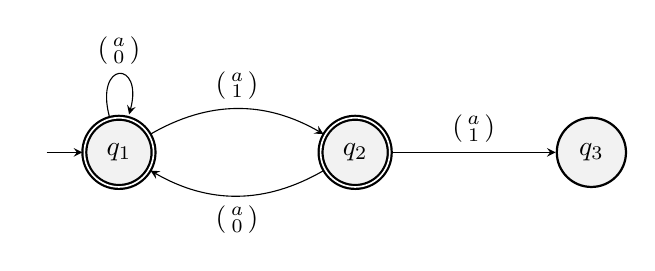
\begin{tikzpicture}
            \node[state, initial, accepting] (q1) {$q_1$};
            \node[state, accepting, right of=q1] (q2) {$q_2$};
            \node[state, right of=q2] (q3) {$q_3$};
            \draw (q1) edge[loop above] node{$\icol{a\\0}$} (q1)
            (q1) edge[bend left, above] node{$\icol{a\\1}$} (q2)
            (q2) edge[bend left, below] node{$\icol{a\\0}$} (q1)
            (q2) edge[above] node{$\icol{a\\1}$} (q3);
            \end{tikzpicture}
        \caption{Deterministic automaton recognizing the same language as expression $\varphi(X)$}
        \label{fig:my_label}
    \end{figure}
\end{example} \

The method we intend to use to prove that 1Q sequences modulo are eventually periodic involves simplifying the 1Q expressions that define such sequences. The primary source of complexity in 1Q expressions is the use of semiring quantifiers. To calculate the values of a sequence defined by an expression such as $\Sigma_X \ \varphi(X)$, it is necessary to determine how many valuations of $X$ make the expression $\varphi(X)$ true for words of varying lengths $1,2,\ldots$.

Fortunately, manipulations of the automata corresponding to expressions with free variables, such as $\varphi(X)$, enable us to create nondeterministic automata that ``count'' the number of valuations for which $\varphi(X)$ is true.

\begin{lemma}
\label{LemElimVar}
    Let $\varphi$ be an MSO expression with a non-empty set of free variables $V = \{v_1, \ldots, v_n\}$. Let $A$ be the corresponding deterministic finite automaton, i.e., the automaton that recognizes the same language as $\varphi$. Both $\varphi$ and $A$ recognize the language $L \subseteq \Sigma_V^*$. A word $(w, \sigma) \in L$ can equivalently be represented as $(w, \sigma(v_1), \ldots \sigma(v_n))$. Let $v_i \in V$. Define the following language over a reduced alphabet (by ``ignoring'' the variable $v_i$): 
    $$L' = \{(w, \sigma(v_1), \ldots, \sigma(v_{i-1}), \sigma(v_{i+1}), \ldots, \sigma(v_n)) \ : \ (w, \sigma(v_1), \ldots \sigma(v_n)) \in L\}$$
    Now, the following holds:
    \begin{enumerate}
        \item $L'$ can be recognized by an automaton $A'$ that is identical to $A$ but defined over the reduced alphabet $\Sigma_{V \setminus \{v_i\}} = \Sigma \times \{0, 1\}^{|V-1|}$. The transitions of $A'$ differ from those of $A$ by simply ignoring variable $v_i$,
        \item The automaton $A'$ can become nondeterministic, and for an arbitrary word
        $$w_{\setminus\{v_i\}} = (w, \sigma(v_1), \ldots, \sigma(v_{i-1}), \sigma(v_{i+1}), \ldots, \sigma(v_n)) \in L',$$ and 
        $$w^{-1}_{\setminus\{v_i\}} = \{(w, \sigma(v_1), \ldots, \sigma(v_{i-1}), x, \sigma(v_{i+1}), \ldots, \sigma(v_n)) \in L \ : \ x \in \{0, 1\}^* \},$$
        it holds that $nRuns_{A'}(w_{\setminus\{v_i\}}) = |w^{-1}_{\setminus\{v_i\}}|$. This means that the number of accepting runs of the automaton $A'$ for a given valuation of the variables (ignoring the removed variable $v_i$) corresponds to the number of accepting valuations of this variable, given the valuations of the remaining variables in the original language $L$.
    \end{enumerate}
\end{lemma}

\begin{proof} \

    \begin{enumerate}
        \item $A'$ is simply an automaton that recognizes the projection of $\Sigma_V^*$ onto $\Sigma_{V \setminus \{v_i\}}$, effectively ignoring the dimension corresponding to variable $v_i$.
        \item We can demonstrate that $A'$ can become nondeterministic as follows. Let $\delta_A$ be the set of transitions of automaton $A$. Consider three states $q_1, q_2, q_3 \in Q_A$ such that:
        $$q_1 \xrightarrow{(a, v_1, \ldots, v_{i-1}, 0, \ldots v_n)} q_2 \in \delta_A,$$ 
        $$q_1 \xrightarrow{(a, v_1, \ldots, v_{i-1}, 1, \ldots v_n)} q_3 \in \delta_A.$$
        From this construction, it follows that in $A'$, the following transitions occur:
        $$q_1 \xrightarrow{(a, v_1, \ldots, v_{i-1}, \ldots v_n)} q_2 \in \delta_{A'},$$ 
        $$q_1 \xrightarrow{(a, v_1, \ldots, v_{i-1}, \ldots v_n)} q_3 \in \delta_{A'},$$
        which implies that $A'$ is nondeterministic. If no such states exist in $A$ then $A'$ remains deterministic. 
        
        Now, we have to prove that $nRuns_{A'}(w_{\setminus\{v_i\}}) = |w_L|$ for $w_{\setminus\{v_i\}} \in L'$. This follows directly from the construction of $A'$: for every accepting path of $w_{\setminus\{v_i\}}$ in automaton $A'$, there corresponds a valuation of $v_i$ such that automaton $A$ would accept the word $(w, \sigma(v_1), \ldots, \sigma(v_{i-1}), \sigma(v_i), \sigma(v_{i+1}), \ldots, \sigma(v_n))$.
    \end{enumerate}
\end{proof}

\begin{example}[Fibonacci, continued]
\label{ExFibCont}
    Let us continue working on~\cref{ExFib}. There, we considered the following expression with a free variable $X$:
    $$\varphi(X) = \neg(\exists_{x_1}\exists_{x_2} \ x_1 \in X \land x_2 \in X \land x_2 > x_1 \land \neg(\exists_{x_3} \ x_3 > x_1 \land x_3 < x_2 ))$$
    We also constructed a deterministic automaton that recognizes a language over the extended alphabet $\Sigma_V = \{a\} \times \{0,1\}$. From~\cref{LemElimVar}, we know that it is possible to build an automaton, potentially nondeterministic, that ignores one of the free variables, with its number of runs corresponding to the number of valuations of the ignored variable. In this case, this results in the automaton presented in~\cref{fig:my_label2}.

    \begin{figure}[ht]
        \centering
        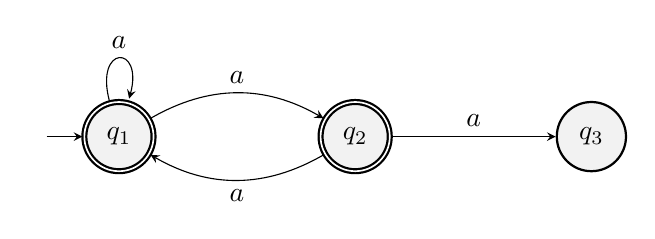
\begin{tikzpicture}
            \node[state, initial, accepting] (q1) {$q_1$};
            \node[state, accepting, right of=q1] (q2) {$q_2$};
            \node[state, right of=q2] (q3) {$q_3$};
            \draw (q1) edge[loop above] node{$a$} (q1)
            (q1) edge[bend left, above] node{$a$} (q2)
            (q2) edge[bend left, below] node{$a$} (q1)
            (q2) edge[above] node{$a$} (q3);
            \end{tikzpicture}
        \caption{Nondeterministic ``counting'' automaton that skips variable $X$ from $\varphi(X)$}
        \label{fig:my_label2}
    \end{figure}

    From the explanation in~\cref{ExFib} regarding the correspondence between $\varphi(X)$ and Fibonacci numbers, and the results in~\cref{LemElimVar}, it follows that the number of accepting runs of the automaton shown in~\cref{fig:my_label2} for a word of length $n$ (i.e., $a^n$) should equal $F(n+2)$. This is indeed the case and can be proven by induction.
\end{example}

The following lemmas are crucial for the elimination of semiring quantifiers in 1Q expressions:

\begin{lemma}
    \label{QuantElimAdd}
    Let $\mathbb{Z}_m$ be a modulo semiring, and let $\varphi$ be a simple recognizable step function on this semiring. Then $\Sigma_x \ \varphi$ and $\Sigma_X \ \varphi$ are also simple recognizable step functions.
\end{lemma}

\begin{proof}
    Since $\varphi$ is a simple recognizable step function, it can be expressed as $\varphi = \sum_{i = 1}^{n} \ \varphi_{L_i} \cdot k_i$, where $\varphi_{L_i}$ are MSO expressions and $k_i \in \mathbb{Z}_m$. Now, consider the expression $\Sigma_{X} \ \varphi$, where $X$ is either a first-order or second-order variable. The reasoning is the same regardless of whether we work with first-order or second-order variables, so we will handle both simultaneously. Some of the MSO expressions inside $\varphi$ might contain $X$ as a free variable, while others might not. Nevertheless, in the semantics of QMSO, $\Sigma$ will iterate over all valuations of $X$ to evaluate this expression. We can assume that every MSO expression inside $\varphi$ contains $X$ as a free variable, by simply concatenating every expression with the always true expression $X = X$.

    Now, for each MSO expression $\varphi_{L_i}$ that appears within $\varphi$, assign a deterministic finite automaton that recognizes the language $L_i$. These MSO expressions include the free variable $X$, so the corresponding automata are defined over an extended alphabet $\Sigma_V$. By having deterministic automata over this extended alphabet, we can apply~\cref{LemElimVar} to construct possibly nondeterministic ``counting'' automata $A_{L_i}$ over alphabet $\Sigma_{V \setminus \{X\}}$. The number of runs of these new automata corresponds to the number of accepting valuations of free variable $X$.

    To handle addition - the semiring quantifier $\Sigma$ - it is sufficient to determine how many times (modulo $m$) each constant $k_i$ appears. To do this, count the number of runs (valuations) for the automaton $A_{L_i}$ using~\cref{CountRunsAutomaton}. For each $A_{L_i}$ and every $k < m$, create an automaton represented by the MSO expression $\varphi_{L_i}^k$ that accepts words over the alphabet $\Sigma_{V \setminus \{X\}}$ for which the number of accepting runs in the original automaton was equal to $k \mod m$. With these automata in place, the addition quantifiers can be eliminated as follows:
    $$\Sigma_X \ \varphi = \sum_{i = 1}^n \sum_{j = 0}^{m-1} \ \varphi_{L_i}^j \cdot (j \cdot k_i \mod m).$$
    $\varphi_{L_i}^j$ can be true for at most one $j$, $0 \leq j \leq m-1$. This $j$ represents the number of successful runs modulo $m$, meaning the number of valuations of $X$ for which $\varphi_{L_i}$ was true. In the original expression, $k_i$ would be added for each such valuation, resulting in $j \cdot k_i$ for this part of the expression. Since we are working modulo $m$, each of these values is taken modulo $m$.
\end{proof}

\begin{lemma}
    \label{QuantElimMult}
    Let $\mathbb{Z}_m$ be a modulo semiring, and let $\varphi$ be a simple recognizable step function over this semiring. Then $\Pi_x \ \varphi$ and $\Pi_X \ \varphi$ are also simple recognizable step functions.
\end{lemma}

\begin{proof}
    Since $\varphi$ is a simple recognizable step function, it can be expressed as $\varphi = \sum_{i = 1}^{n} \ \varphi_{L_i} \cdot k_i$, where $\varphi_{L_i}$ are MSO expressions and $k_i \in \mathbb{Z}_m$. The proof for this lemma will use reasoning similar to that in~\cref{QuantElimAdd}, but with additional complexity. Again, we need to determine how many times each constant $k_i$ appears across all valuations of the variable bound by the quantifier. However, unlike the addition case, it is insufficient to know how many times this constant appears modulo $m$, because in the case of exponentiation, different numbers have different periods when taken modulo $m$. 
    
    For example, consider the constant $2$ when working modulo $3$. We have $2^1 \mod 3 = 2$, $2^2 \mod 3 = 1$, $2^3 \mod 3 = 2$, and so on. For odd exponents, the value will always be $2$, and for even exponents, it will be $1$. Therefore, in this case, we need to know the number of valuations modulo $2$ rather than modulo $3$. 

    The situation is also different for constants that are roots of any order of $m$. Suppose we are working modulo $m = 16$ and have a constant $k_i = 2$. In this case, $2^1 \mod 16 = 2$, $2^2 \mod 16 = 4$, $2^3 \mod 16 = 8$, $2^4 \mod 16 = 0$, $2^5 \mod 16 = 0$, and so on. Thus, after reaching $2^4$, for all subsequent exponents, the value will be $0$. In this case, we observe a prefix sequence $2,4,8$, followed by a constant sequence of $0$.

    The general case is as follows. Consider a constant $k_i$, which we exponentiate modulo $m$. The sequence $Exp_{k_i} = (k_i)^1 \mod m, (k_i)^2 \mod m, (k_i)^3 \mod m \ldots$ is eventually periodic. This follows from the fact that this sequence can take on at most $m$ different values, and once $(k_i)^{n_i} \mod m = (k_j)^{n_j} \mod m$, it implies that $(k_i)^{n_i + 1} \mod m = (k_j)^{n_j + 1} \mod m$ (i.e., once a cycle is reached, it cannot be escaped). Since this sequence is eventually periodic, there exist $N_i, p_i \in \mathbb{N}$, with $p_i > 0$ such that $\forall_{n > N_i} \ Exp_{k_i}(n) = Exp_{k_i}(n + p_i)$. Thus, there is a prefix of length $N_i$ (which may be empty if $N_i = 0$) followed by a repeating cycle of length $p_i$. 

    To determine the influence of the constant $k_i$ on the entire expression, we need to introduce $N_i + p_i$ new constants and MSO expressions. First, for $0 < j \leq N_i$, introduce a constant $k_i^j = (k_i)^j \mod m$ and an MSO expression $\varphi_{L_i}^j$ that asserts the existence of exactly $j$ different valuations of $X$ for which $\varphi_{L_i}$ is true, i.e., $\varphi_{L_i}^j = \exists^{=j} \ \varphi_{L_i}$. This handles the prefix of length $N_i$.
    
    Next, for $N_i < j \leq N_i + p_i$, introduce a constant $k_i^j = (k_i)^j \mod m$ and an MSO expression $\varphi_{L_i}^j$ that asserts there are more than $N_i$ different valuations of $X$ for which $\varphi_{L_i}$ is true, with the number of these valuations being congurent to $j \mod p_i$. For the second property, use the automaton that counts the number of runs modulo, as described in~\cref{CountRunsAutomaton}, in the same way we did in the addition case in~\cref{QuantElimAdd}.

    We also need to address the special case when the constant $k_i$ has no influence on the overall expression, that is, when $\varphi_{L_i}$ is false for every valuation of $X$. To handle this case, introduce $k_i^0 = 1$ (neutral element of multiplication) and $\varphi_{L_i}^0 = \neg(\exists_X \ \varphi_{L_i})$.

    From the construction described, the value corresponding to a constant $k_i$ in the original expression, after quantifier elimination, is given by $\sum_{j = 0}^{N_i + p_i} \ (\varphi_{L_i}^j \cdot k_i^j)$. The inner MSO expression $\varphi_{L_i}^j$ will be true for exactly one $j$.
    
    Now, the multiplication quantifiers can be removed in the following way:
    $$\Pi_X \ \varphi = \prod_{i = 1}^n \ \sum_{j = 0}^{N_i + p_i} \ \varphi_{L_i}^j \cdot k_i^j.$$
\end{proof}

Finally, we can characterize 1Q sequences over a modulo semiring as simple recognizable step functions:

\begin{lemma}
    \label{OverModAreSimpleRec}
    Let $\mathbb{Z}_m$ be a modulo semiring, and let $\varphi$ be a 1Q sentence over $\mathbb{Z}_m$. Then the sequence defined by $\varphi$ can be expressed as a simple recognizable step function (i.e., $\varphi$ can be reduced to the form of a simple recognizable step function). 
\end{lemma}

\begin{proof}
    We proceed by induction on the structure of the expression $\varphi$. For the base case - expressions without quantification at the semiring level - this follows from~\cref{QFreeRecognizable} and~\cref{RecEqSimpleRec}. 
    
    The sum and product of two simple recognizable step functions are also simple recognizable step function - this follows from the induction step of proof of~\cref{DefRecStepFun} and from~\cref{RecEqSimpleRec}.

    Consider an expression $\varphi = Q_Y \ \theta$, where $\theta$ is a simple recognizable step function, $Q$ is a semiring quantifier and $Y$ is either a first-order or second-order variable. By lemmas~\ref{QuantElimAdd} and~\ref{QuantElimMult}, it follows that $\varphi$ is a simple recognizable step function. This completes the proof.
\end{proof}

\begin{fact}
    \label{InvAreReg}
    Let $S$ be a power series defined by a simple recognizable step function $S = \sum_{i = 1}^{n} \ \varphi_{L_i} \cdot k_i$. The language of words for which $S$ achieves the value $k_i$ is precisely the language recognized by $\varphi_{L_i}$ (which is a regular language).
\end{fact}

\begin{proof}
    This follows directly from the definition of a simple recognizable step function and the fact that $\varphi_{L_i}$ is an MSO expression.
\end{proof}

From these results, an important characterization of 1Q sequences over modulo semirings follows: 1Q sequences over modulo semirings are eventually periodic.

\begin{lemma}
    \label{OverModAreSimpleRec2}
    Let $\mathbb{Z}_m$ be a modulo semiring and let $\varphi$ be a 1Q sentence over $\mathbb{Z}_m$. Then the sequence defined by $\varphi$ is eventually periodic.
\end{lemma}

\begin{proof}
    Thanks to~\cref{OverModAreSimpleRec}, we know that $\varphi$ reduces to a simple recognizable step function. Additionaly, by~\cref{InvAreReg}, we know that the language of words for which the sequence defined by $\varphi$ achieves a given value $k_i$ is a regular language. Since there is a finite number of values this sequence can achieve (at most $m$). Regular languages on one-letter alphabets are eventually periodic with regard to word length (\cite[Theorem 1]{PighizziniS02}).

    There are $m$ regular, disjoint languages $L_1, \ldots, L_m$ corresponding to different constants $k_i$. We assume these languages do not accept the empty word. Each language $L_i$ is eventually periodic with respect to word length, so there exist $N_i, p_i \in \mathbb{N}$ such that $\forall_{n \geq N_i} \ a^n \in L_i \iff a^{n + p} \in L_i$. To find a ``global'' period that works for all langauges, take $N = \prod_{i=1}^m \ N_i$ and $p = \prod_{i=1}^m \ p_i$. This period serves as a common period for every $L_i$ since $N$ is a multiple of each $N_i$ and $p$ is a multiple of each $p_i$.
\end{proof}

From this, the main result of this section,~\cref{1QSequencesPeriodic}, follows directly

\begin{proof}[Proof of~\cref{1QSequencesPeriodic}]
    1Q sequences modulo are equivalent to 1Q sequences over a modulo semiring (\cref{1QModulo}). Thus, the result follows directly from~\cref{OverModAreSimpleRec2}.
\end{proof}

\begin{corollary}
    Catalan numbers are not 1Q-definable
\end{corollary}

\begin{proof}
    The reasoning is the same as in~\cite[Theorem 7, Corollary 8]{CadilhacMPPS20}, which uses results about Catalan sequences from~\cite{KubotaCatalan}. Catalan numbers are not ultimately periodic modulo sufficiently large prime numbers, while 1Q-definable sequences are. Therefore, Catalan numbers are not 1Q-definable.
\end{proof}

\section{Other Topic of Interest}
\label{SecOther}
During the research on 1Q sequences, several other interesting topics emerged, though they were not fully explored.

\subsection*{Characterization of 1Q sequences}
\label{CharacterizationOf1QSequences}
1Q expressions a broad class of sequences, notably including the entire class of linear recursive sequences. An interesting research question is: what precisely is the class of sequences defined by 1Q expressions? Is there a simpler or alternative representation of these sequences?

In the Introduction, it was noted that 1Q expressions can define sequences that are not polynomial recursive. This raises an interesting question: is every polynomial recursive sequence also 1Q-definable? This question is challenging to answer, as expressing recursion using 1Q expressions is not straightforward.

\subsection*{Complexity of Zero Checking}
When working over a modulo semiring, what is the time complexity $O(|\varphi|)$ of checking whether a sequence defined by such a sentence is constantly equal to zero?

Consider a naive zero-checking procedure that simply iterates over the first $n$ elements of the sequence defined by $\varphi$ and checks whether they are all zero. How many elements must be checked to ensure that the sequence is constantly equal to zero? This problem can also be phrased as: how far into the sequence can the first non-zero element appear, relative to the length of the 1Q expression?

It turns out that this problem has super-exponential complexity, even without semiring quantifiers. This complexity arises from the expressive power of MSO. In MSO, it is possible to define a sentence of length $n$ that does not accept words of length smaller than $tower(n)$ (citation needed). The function $tower$ is defined recursively as $tower(0) = 2$ and $tower(n) = 2^{tower(n-1)}$.

\subsection*{1Q on first-order logic}
The task of characterizing 1Q sequences is non-trivial, but it may be interesting to look into a restriction of 1Q expressions where we only use first-order variables at both the semiring and logical level (i.e., moving from monadic second-order logic to first-order logic).

Unfortunately, this class of sequences also appears challenging to characterize, and it is not obvious how to determine whether a given sequence is definable as a 1Q sentence in first-order logic.

Instead, it might be worthwhile to revisit sequences modulo, as we did in~\cref{Sec1QFiniteSemirings}.

As stated in~\cite{DrosteG07}, first-order definable series coincide with series definable by weighted automata when working with aperiodic semirings. Unfortunately, the semirings we are working with - modulo semirings - are not aperiodic. This can be illustrated by the sequence defined by the following expression:

$$ \Sigma_x \ . \ 1 $$

This defines the following sequence modulo 2: $\{1, 0, 1, 0, 1, \ldots\}$, which is not aperiodic. An interesting aspect of this sequence is that the languages of words for which it achieves specific values are not first-order definable. For instance, it achieves the value $1$ for words of odd lengths ($1, 3, 5, \ldots$). Such a language is not first-order definable. Therefore, even though we restrict the expressions to first-order logic, additional complexity is introduced by the semiring operations.

We might want to ask if it is possible to define following sequence in 1Q modulo $2$ using first-order logic: $\{0, 0, 1, 0, 0, 1, \ldots\}$, where the ones appear on positions divisible by 3. It seems unlikely, and it might be provable that the only sequences definable modulo 2 are those with periods that are powers of $2$.

\bibliographystyle{plainurl}
\bibliography{bib}

\end{document}
